\documentclass[12pt]{article}
\usepackage{graphicx}
\def\key#1{{\bf #1}}

\begin{document}
\title{How the GUIB works}
\author{Anton Kokalj}
\maketitle
\begin{abstract}
  This document describes briefly the GUIB: (i) how it works, and (ii)
  how to make a GUI application by using the GUIB engine. It is highly
  recommended that the document from the GUIB web page entitled {\em
    Description} is read first.
  \\[1em]
%  {\bf BEWARE:} this document is in under preparation ...
\end{abstract}

\tableofcontents

\section{The easiest way}

The easiest way to create a simple GUI application, is to use the {\tt
  guib} script that comes with GUIB package. Let say that your module
definition-file is named {\tt myGUI.def}, then a simple GUI will be
constructed by the following execution: 
\begin{verbatim}
guib myGUI.def 
\end{verbatim}

To explain how the {\tt guib} script works, the following diagram is
provided:

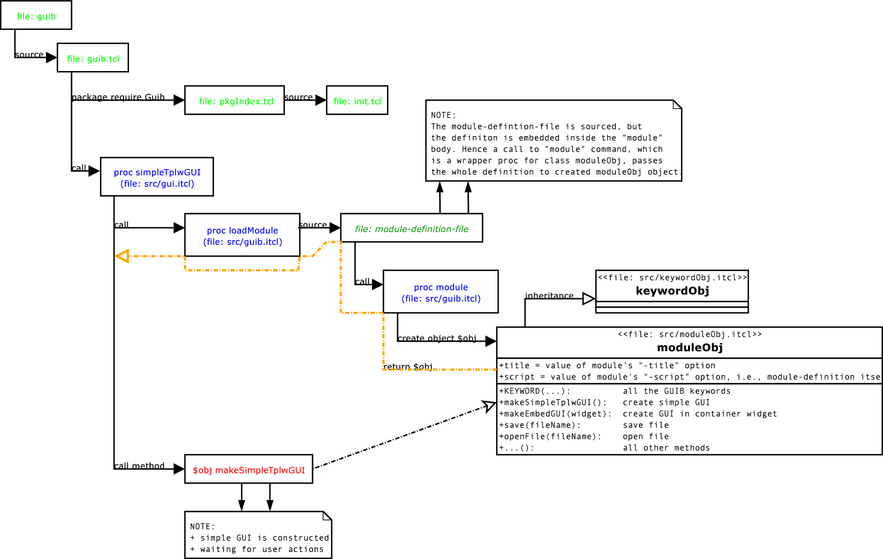
\includegraphics[width=1.0\textwidth]{diagrams/Guib.png}

This diagram shows that the module definition-file is source from the
\key{loadModule} procedure. Technically, the module definition-file is
a Tcl script, which uses the GUIB library. The whole script is
embedded inside the \key{module} keyword, which is a wrapper for the
\key{moduleObj} class. This means that by a call to \key{module} an
object of \key{moduleObj} type is constructed. This is a complex
object, and it holds the whole GUI definition.

To illustrate---from programming point of view---how the definition of
the GUI is stored in the \key{moduleObj} type object, let us consider
the following example:

{\small
\begin{verbatim}
module \#auto -title "Testing" -script {
    page p1 -name "Page No.1" {
        line l1st -name "1st line" {
            var title -label "Title:"
            var code  -label "Code:"
        }
        line l2nd -name "2nd line" {
            var description -label "Description:"
        }
    }
    line llast -name "last line" {
        var conclusion -label "Conclusion:"
    }
}
\end{verbatim}
}

Here the following GUIB keywords are used: \key{module}, \key{page},
\key{line}, \key{var}. The GUIB keywords can be divided into two
groups: objects and items. The keywords such as \key{page} and
\key{line} are object-keywords as they construct new object of a given
type, while the \key{var} keyword is an example of the item-keyword,
i.e., item keywords do not create new objects, but their content is
stored in corresponding object-keyword. Which GUIB keyword is object-
or item-like can be guessed from the syntax. Consider the following:
{\small
\begin{verbatim}
line l1st -name "1st line" {
    var title -label "Title:"
    var code  -label "Code:"
}
\end{verbatim}
} Obviously, the \key{line} keyword is an object-keyword, and in this
examples it holds two \key{var} item-type keywords.

The base-class of keyword objects is \key{keywordObj} class. This
class possesses a mechanism for storing the information of the module
definition file in hierarchical fashion. Let say that we want to
retrieve all information of the module definition file that was
already stored in \key{moduleObj} type object. This will be done
recursively and will look like this:

{\small
\begin{verbatim}
proc retrieve_and_DoWhatever {obj} {

    set NItem [$obj getID]   
    for {set id 0} {$id <= $NItem} {incr id} {        

        # check if $id keyword is object-type !!!
        set childObj [$obj getChild $id]
        
        if { $childObj != "" } {
            #
            # keyword is OBJECT-type, manage it recursively
            #
            ...
            retrieve_and_DoWhatever $childObj
            ...
        } else {
            #
            # keyword is ITEM-type 
            #
            ...
        }
    }
}
\end{verbatim}
}
To illustrate more schematically, how the information about the
module-definition file is stored, the following diagram shows
this graphically for the above \key{module \#auto -title "Testing"
  -script \{...\}} example.

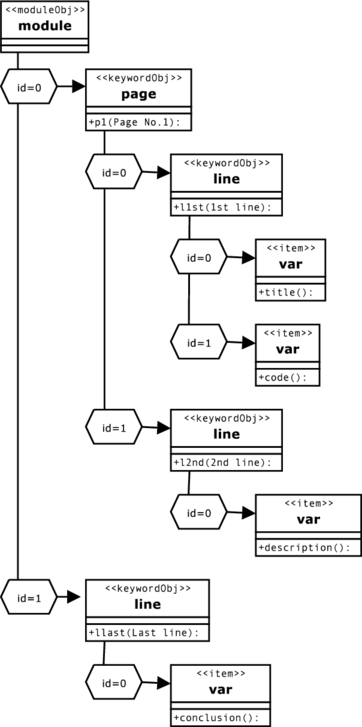
\includegraphics[width=0.5\textwidth]{diagrams/parsing.png}


\section{A more elaborate way}

The GUI constructed by the {\tt guib} script can only hold one module
definition file. Moreover no configuration is possible. If we want to
create a configurable GUI that will be able to create/manipulate
several different input files, than a \key{GUI} class provided by the
GUIB package can be used. Below scheme shows the idea in diagrammatic
fashion:

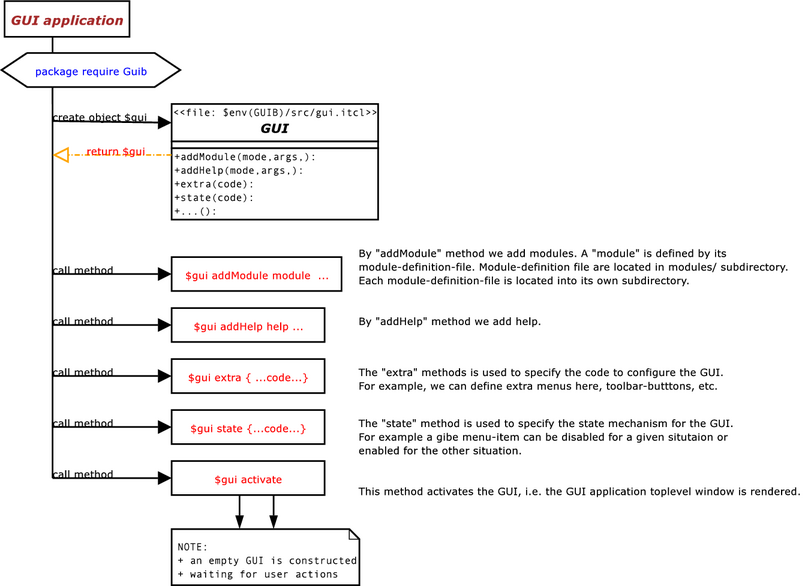
\includegraphics[width=1.0\textwidth]{diagrams/myGUI.png}

Now let us do a sample GUI application that will use the \key{GUI}
class to construct a configurable GUI, which will be able to
create/manipulate several input files. Let's say that the module
definition files for these inputs are stored in files {\tt
  myInput-1.def}, and {\tt myInput-2.def}. Let's say we also have help
files with description of both input formats stored in files {\tt
  myInput-1.html}, and {\tt myInput-2.html}. Now we have to create a
GUI script, for example:

{\footnotesize
\begin{verbatim}
#!/bin/sh
# next line restarts wish \
exec wish

# ------------------------------------------------------------------------
#  INITIALIZATION
# ------------------------------------------------------------------------

# check if GUIB environmental variable is defined

if { [info exists env(GUIB)] } {
    # instruct the Tcl where to search for GUIB package
    lappend auto_path [file join $env(GUIB)]
} else {
    # we assume that GUIB package is on some "standard" path and Tcl
    # will find it.
}

# load a Guib package
package require Guib 0.1.1

# withdraw the "." toplevel window, and bind the <Destroy> event
# to ::guib::exitApp
wm withdraw .
bind . <Destroy> ::guib::exitApp


# ------------------------------------------------------------------------
#  GUI construction
# ------------------------------------------------------------------------

# construct the GUI object
set gui [::guib::GUI \#auto -title "My 1st GUI" -appname MyGUI]

# Add modules. The syntax is:
# ------------
# $gui addModule module $moduleID $moduleLabel $moduleFile
#
$gui addModule module inp1 "My Input-1" myInput-1.def
$gui addModule module inp2 "My Input-2" myInput-2.def

# Add help. The syntax is:
# ---------
# $gui addHelp help $helpID $helpLabel $helpFile
#
$gui addHelp help help1 "Help for Input-1" myInput-1.html
$gui addHelp help help2 "Help for Input-2" myInput-2.html


#
# some extra configuration of the GUI
#
$gui extra {
    #
    # add a logo to toolbar panel
    #
    image create photo myLogo -format gif -file myLogo.gif

    set tb   [component toolbar]
    set logo [$tb add label logo -image myLogo]
    pack configure $logo -side right
}
\end{verbatim}
}

When GUI defined in above file will be launched, an application
toplevel window with menubar and toolbar will appear. But none of the
GUI will be rendered. This can be done by selecting either \key{File
  $\rightarrow$ New Input ...} or \key{File $\rightarrow$ Open Input
  ...} menu. The following diagram shows a programming scheme for
\key{New Input ...} method:

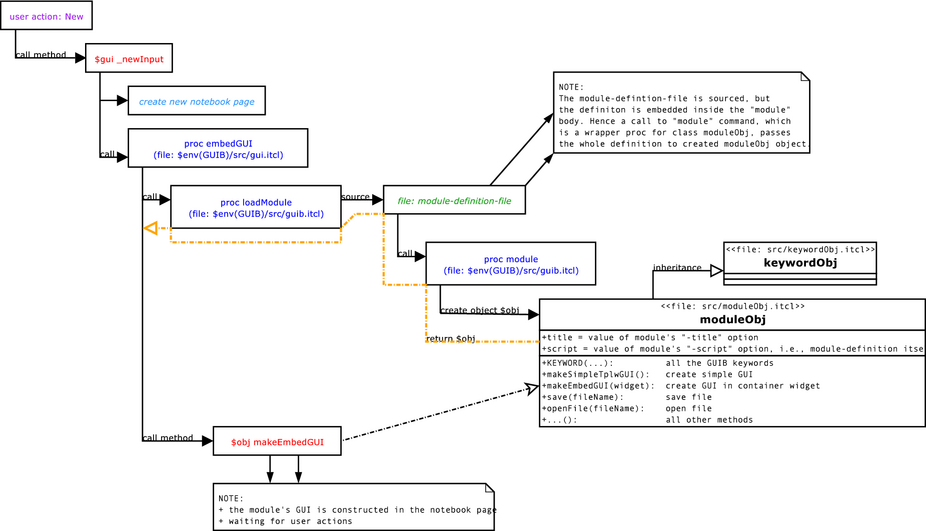
\includegraphics[width=1.0\textwidth]{diagrams/GUI-new.png}

The scheme for the \key{Open Input ...} is very similar. In fact the
``open'' method first call the ``new'' method, which constructs an
appropriate GUI, and then an existing file is loaded in that GUI. The
scheme is shown here:

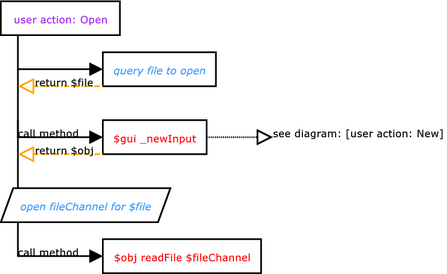
\includegraphics[width=.5\textwidth]{diagrams/GUI-open.png}

\section{An example of real GUI application: PWgui}

PWgui is a GUI for PWscf set of numerical programs for electronic
structure calculations. It is a real GUI application that uses the
GUIB engine. It is only a slightly more complicated than above GUI
example.  Here is a diagram showing the structure of the PWgui
application:

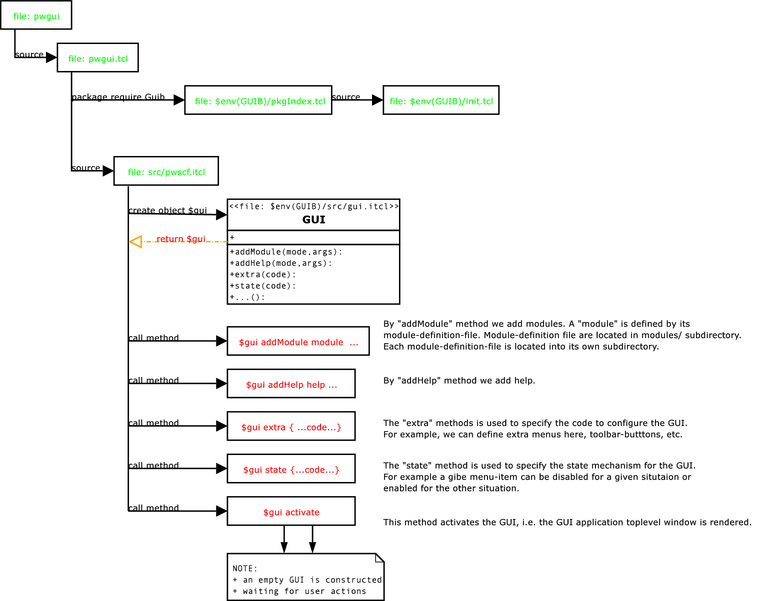
\includegraphics[width=1.0\textwidth]{diagrams/PWgui.png}

\section{File and directory structure of GUIB}

\begin{description}
\item[Directory structure:]~\\
  \begin{tabular}[t]{ll}
    $\bullet$~\tt lib/      & auxiliary Tcl/Tk routines, i.e., tclUtils.tcl, tkUtils.tcl\\
    $\bullet$~\tt doc/      & programming documentation generated from source-code\\
    $\bullet$~\tt examples/ & a few examples (definition files: *.tcl; input files: *.inp)\\
    $\bullet$~\tt external/ & external \key{cmdline} library\\
    $\bullet$~\tt images/   & \\
    $\bullet$~\tt src/      & GUIB source code directory\\
  \end{tabular}
\item[Description of some src/ files:]~\\
  \begin{tabular}[t]{ll}
    $\bullet$~\tt moduleObj.itcl    & implementation of \key{moduleObj} class\\
    $\bullet$~\tt keywordObj.itcl   & implementation of \key{keywordObj} class\\
    $\bullet$~\tt guibKeywords.itcl & implementation of all GUIB keywords\\
    $\bullet$~\tt build.itcl        & build Tk-based GUI defined by module definition file.\\
    $\bullet$~\tt open.itcl         & open an input file\\     
    $\bullet$~\tt save.itcl         & save edited input file\\[1em]    
    $\bullet$~\tt guib-keywords-def.tcl & definition of options of GUIB-keywords\\[1em]
    $\bullet$~\tt gui.itcl          & application GUI: procs for "simple-GUI" and\\
                                    & implementation of more elaborate \key{GUI} class\\[1em]
  \end{tabular}
\end{description}
\end{document}

%%% Local Variables: 
%%% mode: latex
%%% TeX-master: t
%%% End: 
